\begin{problem}{가장 높고 넓은 성}
    {표준 입력}{표준 출력}
    {1 초}{512 MB}{}
    
    
    
    당신은 어마어마한 크기의 토지를 소유한 부자다. 평지에는 $ n $개의 표지판이 있다. 당신은 지금부터 이 곳에 민성이를 위한 성을 지을 것이다. 성은 여러 개의 층으로 구성된 구조물이다.
    
    \begin{itemize}
        \item 1층은 평지 위에 지어지고, 2층은 1층 위에, 3층은 2층 위에, $ \cdots $, $ n $층은 $ n-1 $층 위에 지어진다.
        \item 각 층의 경계는 다각형이며, 각 층의 경계의 꼭짓점에는 표지판이 위치하여야 한다. 다시 말하면, 표지판 위에만 각 층의 경계의 꼭짓점을 세울 수 있다.
        \item 한 표지판은 여러 층의 경계의 꼭짓점에 동시에 사용될 수 없다. 그러나 한 표지판이 다른 층의 꼭짓점이 아닌 경계에 위치할 수는 있다.
        \item 넓이가 0인 층은 허용되지 않는다.
        \item 쓸모가 없는 표지판들은 버려도 된다.
    \end{itemize}
    민성이는 숙소를 고를 때 전망을 최우선으로 고려하므로, 당신이 성을 지을 때 고려해야 할 우선순위는 다음과 같다.
    
    \begin{enumerate}
        \item 성의 높이를 가능한 한 제일 높게 지어야 한다.
        \item 성의 모든 층의 넓이의 합이 가능한 한 제일 크게 지어야 한다.
        \item 가능한 적은 수의 표지판을 사용하여야 한다.
    \end{enumerate}
    당신은 성을 몇 층까지 지을 수 있으며, 그 때 각 층에 사용될 표지판들이 무슨 표지판인지 알아내야 한다.
    
    
    \InputFile
    첫 번째 줄에 표지판의 개수 $ n $이 주어진다. ($ 1 \leq n \leq 10^3 $) 
    
    두 번째 줄부터 $ n $개의 줄에 걸쳐 각 표지판들의 위치를 의미하는 정수 $ x $, $ y $가 공백으로 구분되어 주어진다. ($ -10^4 \leq x,\ y \leq 10^4 $) 이는 $ (x, y) $에 표지판이 위치함을 의미한다.
    
    모든 표지판은 서로 다른 위치에 세워져 있다.
    
    
    \OutputFile
    첫 번째 줄에 $ n $개의 정수 $ x_1,\ x_2,\ \cdots,\ x_n $를 공백으로 구분하여 출력한다. $ x_i $는 $ i $번째 표지판이 사용되었을 경우 사용된 층수이며, 사용되지 않았으면 0이다.

    \Examples
    
    \begin{example}
        \exmp{
            9
            0 0
            -1 3
            -1 -2
            -5 -5
            2 -2
            2 2
            3 1
            3 -5
            1 -1
        }{%
            2 1 2 1 2 1 1 1 0
        }%
    \exmp{
            12
            0 0
            1 0
            2 0
            3 0
            4 0
            3 1
            2 2
            1 3
            0 4
            0 3
            0 2
            0 1
        }{%
            1 2 3 2 1 2 3 2 1 2 3 2
        }%
    \end{example}
    
    \Explanation
    첫 번째 예제를 시각화하면 다음과 같다. 마지막 점인 $ (1, -1) $은 사용되지 않았다.
    \begin{figure}[h]
        \centering
        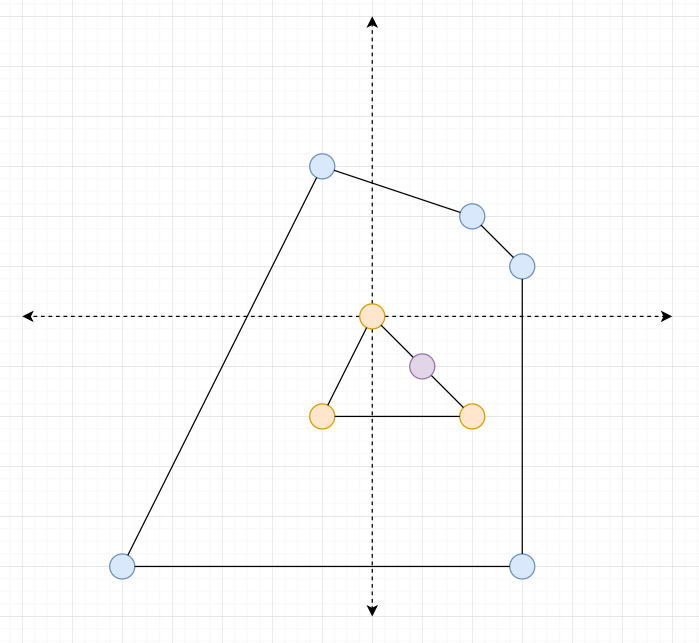
\includegraphics[width=0.35\textwidth]{castle.png}
    \end{figure}
    
\end{problem}

